\section{Результаты}
\label{sec:results}

Для начала проведём вычисления с использованием малости нормы градиента в качестве критерия остановки.

Вычисления проводились для точности $10^{-6}$, параметры дробления метода Пшеничного: $\lambda = 0.9, \epsilon = 0.45$

Далее приведены графики зависимости точности (нормы разности текущего и точного значения) от номера шага и геометрическая интерпретация работы методов (показаны линии уровня и вектора шага).

Здесь и далее, графики в логарифмическом размере выглядят вертикальными, если принимают значение 0 (точное решение).

Зелёный пунктир - заданная точность

\begin{figure}[H]
			\centering
			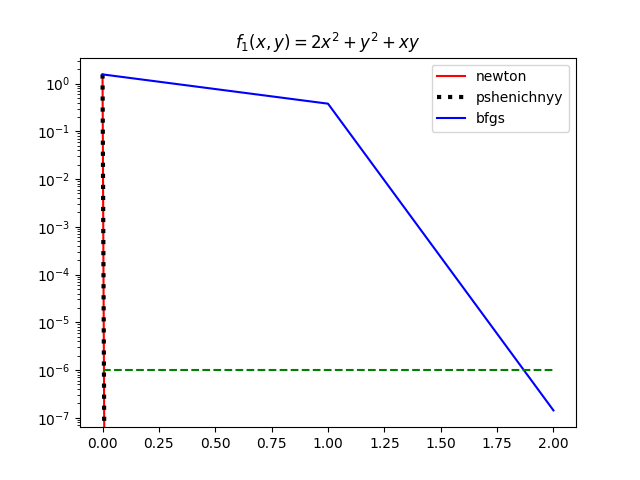
\includegraphics[scale=0.75]{figures/acc_from_step_func1}
			\caption{Точность от шага, $f_1$, критерий - градиент}
			\label{fig:acc_from_step_func1}
\end{figure}

\begin{figure}[H]
			\centering
			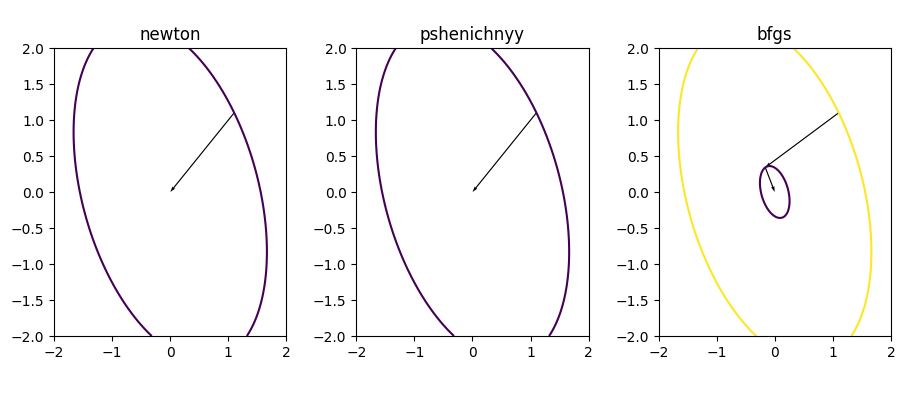
\includegraphics[scale=0.75]{figures/process_view_func1}
			\caption{Иллюстрация работы алгоритмов, $f_1$}
			\label{fig:process_view_func1}
\end{figure}

Как видим, заданная точность достигается всеми алгоритмами, остановка происходит вовремя.
Как и ожидалось, методы второго порядка решили точно за 1 шаг.
Квазиньютоновский метод очень хорошо приблизил решение на втором шаге (сразу после первой корректировки приближения матрицы Гессе)

\begin{figure}[H]
			\centering
			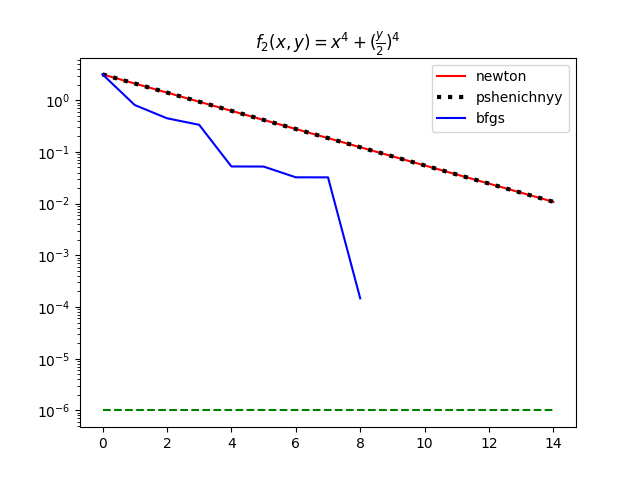
\includegraphics[scale=0.75]{figures/acc_from_step_func2}
			\caption{Точность от шага, $f_2$, критерий - градиент}
			\label{fig:acc_from_step_func2}
\end{figure}

\begin{figure}[H]
			\centering
			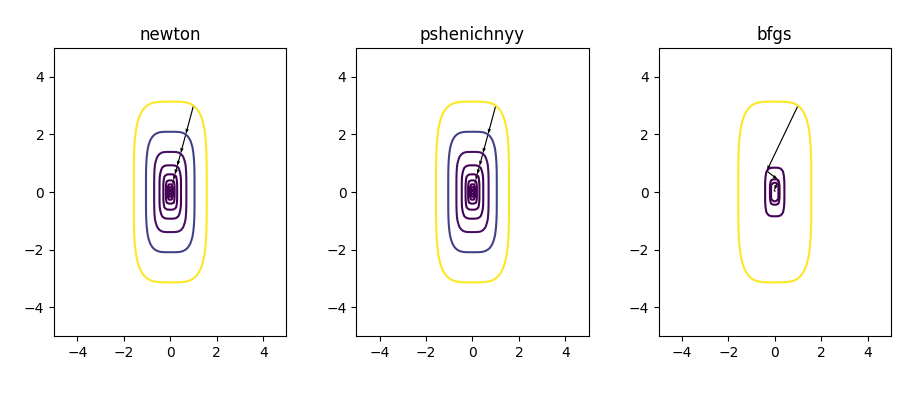
\includegraphics[scale=0.75]{figures/process_view_func2}
			\caption{Иллюстрация работы алгоритмов, $f_2$}
			\label{fig:process_view_func2}
\end{figure}

Заметим, что так как в окрестности точки минимума функция ведёт себя как функция четвёртой степени, градиентная оценка приводит к преждевременной остановке алгоритма.

Также, этот опыт показывает, что данная функция плохо аппроксимируется эллиптическим параболоидом, поэтому методы второго порядка медленно сходятся.
Квазиньютоновский метод в этом случае оказывается быстрее, благодаря оптимальному выбору длины шага.

\begin{figure}[H]
			\centering
			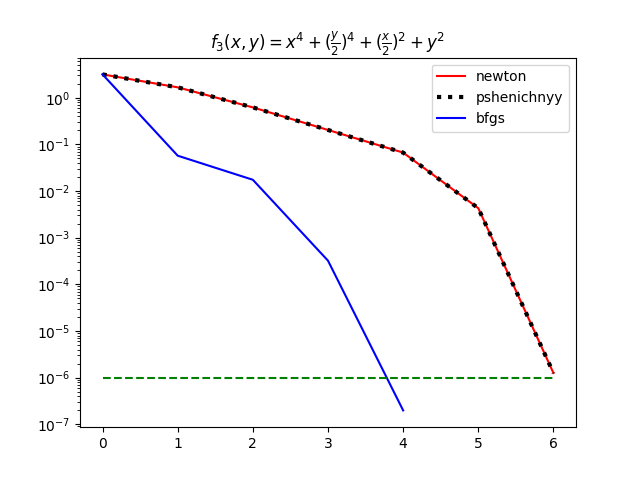
\includegraphics[scale=0.75]{figures/acc_from_step_func3}
			\caption{Точность от шага, $f_3$, критерий - градиент}
			\label{fig:acc_from_step_func3}
\end{figure}

\begin{figure}[H]
			\centering
			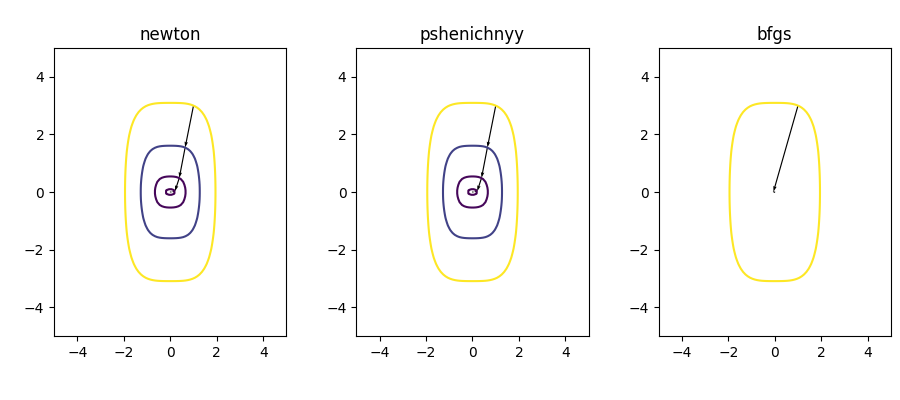
\includegraphics[scale=0.75]{figures/process_view_func3}
			\caption{Иллюстрация работы алгоритмов, $f_3$}
			\label{fig:process_view_func3}
\end{figure}

Видим, что при добавлении к $f_2$ квадратных членов достоверность градиентного критерия улучшилась, хотя и не полностью, так как методы второго порядка хоть и приблизились близко, но не дали заданной точности.

Одновременно с этим, все методы стали сходиться быстрее, но квазиньютоновский метод всё ещё обходит квадратичные.

\begin{figure}[H]
			\centering
			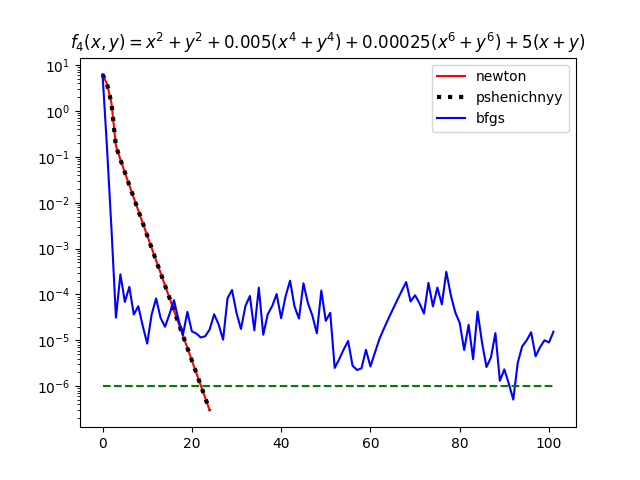
\includegraphics[scale=0.75]{figures/acc_from_step_func4}
			\caption{Точность от шага, $f_4$, критерий - градиент}
			\label{fig:acc_from_step_func4}
\end{figure}

\begin{figure}[H]
			\centering
			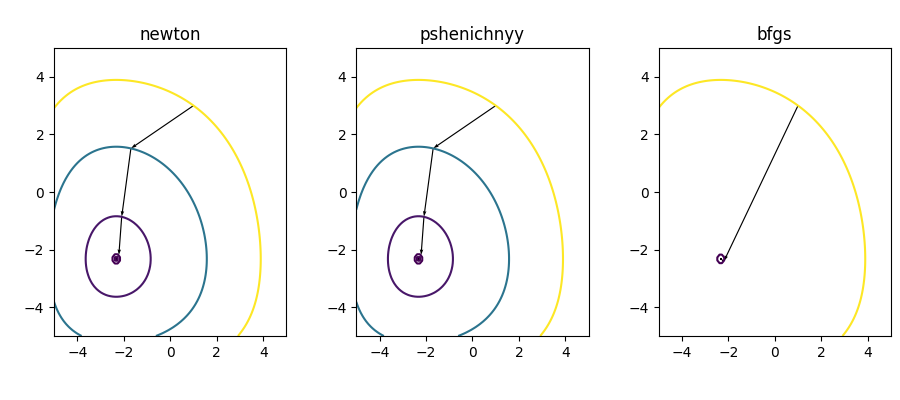
\includegraphics[scale=0.75]{figures/process_view_func4}
			\caption{Иллюстрация работы алгоритмов, $f_4$}
			\label{fig:process_view_func4}
\end{figure}

Как видим, на данной функции квадратичные методы сходятся медленнее, чем в случае $f_3$, а квазиньютоновский и вовсе перестаёт сходиться ближе $10^-4$.

Отметим, что эта функция единственная из рассмотренных с минимумом не в нуле.
Но, проведя исследования этой же функции с перенесённым в точку минимума началом координат, мы увидели абсолютно те же результаты.

Градиентная оценка здесь приводит к нескольким лишним шагам алгоритма.



Как показал этот опыт, на выбранных нами функциях метод Пшеничного всегда выполняет 0 дроблений и вырождается в метод Ньютона, поэтому далее не будем его рассматривать.

В следующем опыте проверим скорость сходимости методов, в зависимости от начального приближения.
Для этого проведём вычисления для 100 точек, равномерно распределённых на окружности с центром в точке минимума и радиусом 2.
На следующих графиках изображена зависимость близости решения от номера шага алгоритма.
В этом опыте критерием остановки взято расстояние до точного решения, так как ранее было показано, что градиентный критерий даёт разные результаты для разных функций.

На рисунках красным обозначены решения методом Ньютона, синим - методом БФГШ.
Зелёным пунктиром отмечена целевая точность $= 10^-6$.

\begin{figure}[H]
			\centering
			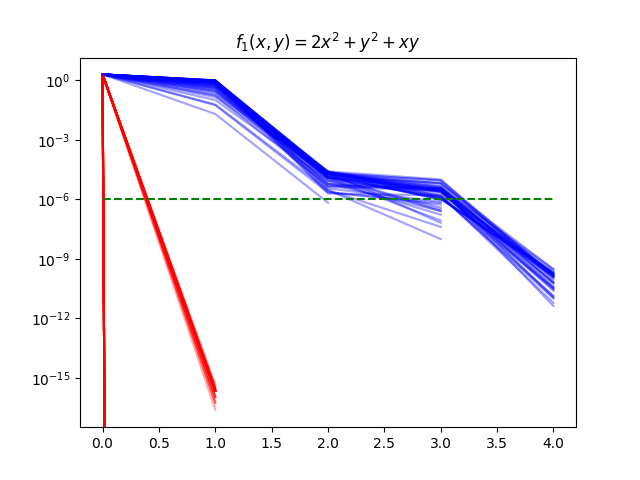
\includegraphics[scale=0.75]{figures/init_100_func1}
			\caption{Выборка начальных приближений, $f_1$}
			\label{fig:init_100_func1}
\end{figure}

Для первой функции метод Ньютона всегда находит решение за 1 шаг, в некоторых случаях - точно (вертикальные линии на графике).
Квазиньютоновскому методу требуется от 2 до 4 шагов.
В среднее число шагов в выборке 3,7.

\begin{figure}[H]
			\centering
			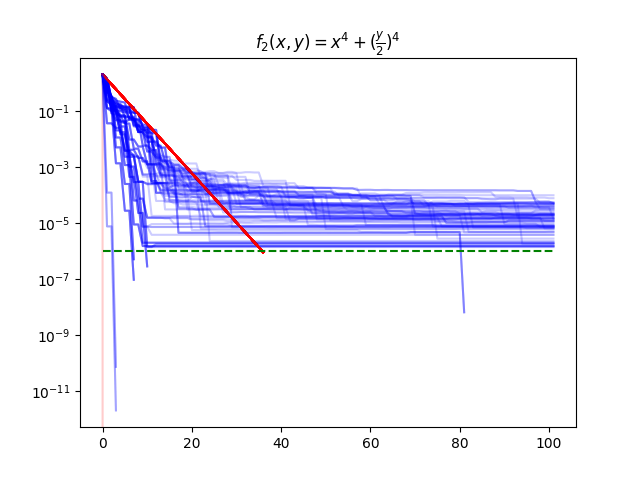
\includegraphics[scale=0.75]{figures/init_100_func2}
			\caption{Выборка начальных приближений, $f_2$}
			\label{fig:init_100_func2}
\end{figure}

Здесь становится видно, квазиньютоновский метод плохо справляется с полиномами 4 степени и не сходится в большинстве случаев.
Метод ньютона же, сходится за 36 шагов, и обладает зависимостью $n = -5,7 log_10(|x_*-x|)$.

\begin{figure}[H]
			\centering
			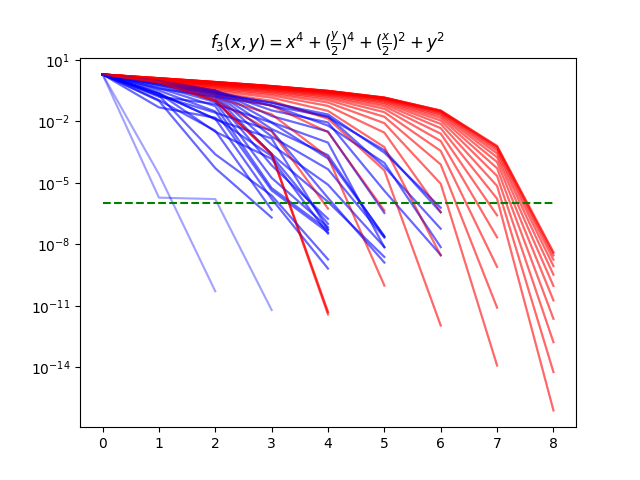
\includegraphics[scale=0.75]{figures/init_100_func3}
			\caption{Выборка начальных приближений, $f_3$}
			\label{fig:init_100_func3}
\end{figure}

При добавлении квадратичных членов оба метода стали хорошо сходиться.
Но при этом, для данной функции наблюдается заметный разброс в скорости сходимости от начального приближения для обоих методов.
Среднее число шагов:

Метод ньютона - 6.76

Метод БФГШ - 4.58

\begin{figure}[H]
			\centering
			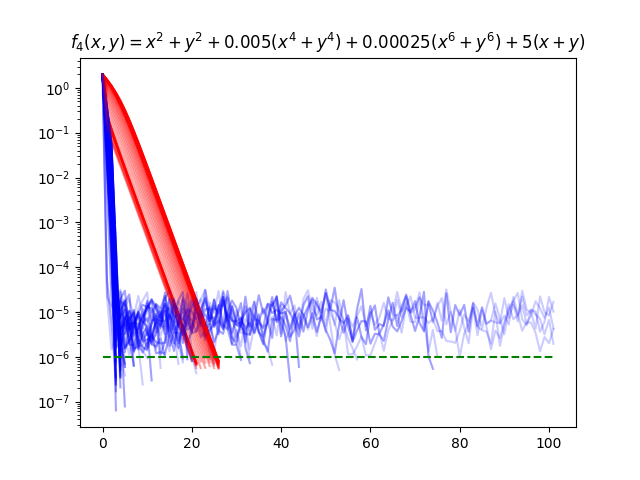
\includegraphics[scale=0.75]{figures/init_100_func4}
			\caption{Выборка начальных приближений, $f_4$}
			\label{fig:init_100_func4}
\end{figure}

Для данной функции снова имеем не сходящийся ближе чем $10^-5$ метод БФГШ и зависимость $n = a+b log_10(|x_*-x|)$.
Однако, в отличие от функции $f_2$, где БФГШ не ухудшал результат, здесь явно видны скачки точности в худшую сторону.
